\section{DRL-Based QOCO Algorithm}
%\subsection{DQN-based solution}
%\subsection{Computation Model}

\begin{frame}
	\frametitle{DQN-based solution}
	\begin{figure}
	\captionsetup{name=Fig.}
	\centering
	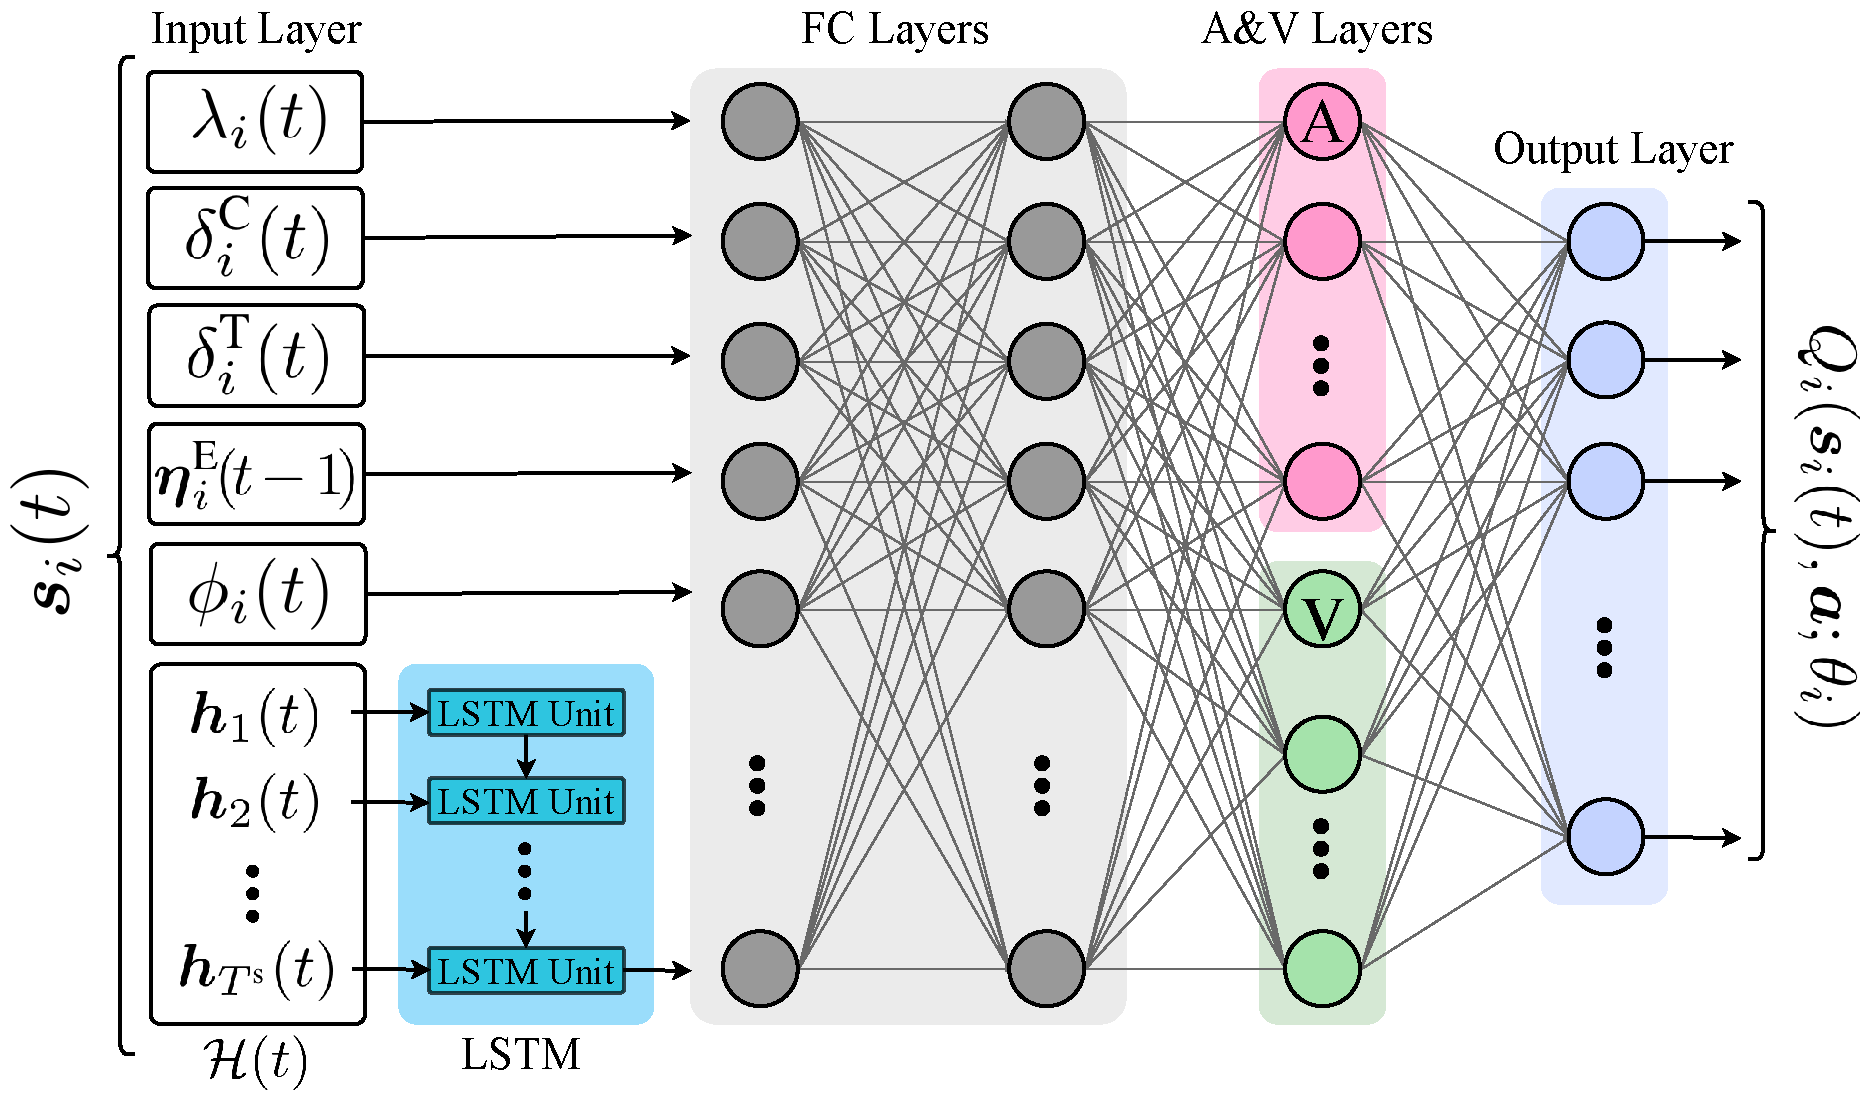
\includegraphics[width=0.9\linewidth]{DQN}
	\vspace*{-5mm}
	%\caption{An illustration MD $i \in \mathcal{I}$ and EN $j \in \mathcal{J}$ in the MEC system.}
	\vspace*{-3mm}
	\label{fig1}
\end{figure}
	
	\vspace{6mm}
	
	\begin{itemize}[]
	
	\item  \hspace{0mm}  \textcolor{teal}{LSTM}: ENs Load Level Prediction
	
	\item  \hspace{0mm}  \textcolor{teal}{FC}: State-Action Q-Value Mapping
	
	
	\item \hspace{0mm}  \textcolor{teal}{A\&V}: Dueling-DQN Approach for Q-Value Estimation
	
	
	
	
\end{itemize}

	
\end{frame}


\begin{frame}
	\frametitle{QOCO Algorithm}
	


	\textbf{Stracture:}
	
	
	\begin{itemize}[]
		\item ENs help MDs to traine their neural networks.
		\item The algorithms to be executed at MD and EN
		\item Training neural networks with MD experiences 

		


			\begin{itemize}{}
			\item \textbf{(i.e., state, action, QoE, next state)} 
		\end{itemize}
		\item Mapping Q-values to each state-action pair
		

	\end{itemize}

\vspace{4mm}

	
	\textbf{In detail:}
	\vspace{1mm}
\begin{itemize}
	\item MD's Neural Network in EN:

	\begin{itemize}{}
		\item \textbf{Replay Memory:} Records the observed experience of MD.
		\vspace{1mm}
		\item \textbf{Evaluation Network:} Responsible for action selection. $Q_i^{\text{E}}(\boldsymbol{s}_i(t), \boldsymbol{a}; \theta^{\text{E}}_i)$ 
			\vspace{1mm}
		\item \textbf{Target Network:} Characterizes the target Q-values. $Q_i^{\text{T}}(\boldsymbol{s}_i(t), \boldsymbol{a}; \theta^{\text{T}}_i)$
			\vspace{2mm}
	\end{itemize}
	\item Updating the evaluation network parameter vector:
	\begin{itemize}
		\item Minimization of the difference between the Q-values under evaluation and target networks.
	\end{itemize}
\end{itemize}
	
	
\end{frame}

\begin{frame}
	\frametitle{QOCO Algorithm}

	\textbf{Offloading Decision Algorithm at MD:}
	\vfill


	
	\begin{itemize}[]
		
		
		\item MD sends an $\textit{UpdateRequest}$ to EN.
		
		\item Receive network parameter vector $\theta_i^{\text{E}}$ from EN
		
		\item Select an Action for each Computation Task based on 
			\begin{alignat}{2}
			\hspace*{-2mm}\boldsymbol{a}_i(t) \hspace*{-0.5mm} = \hspace*{-0.5mm}
			\begin{cases} 
				\text{arg $\max_{\boldsymbol{a}\in \mathcal{A}}Q_i^{\text{E}}(\boldsymbol{s}_i(t), \boldsymbol{a}; \theta^{\text{E}}_i)$,} &		\hspace*{-3mm} \text{with $\boldsymbol{\text{p}}(1 -\boldsymbol{\epsilon})$} \vspace{3mm}\\
				\text{pick an random action from $\mathcal{A}$,} & \hspace*{-3mm} \text{with $\boldsymbol{\text{p}}(\boldsymbol{\epsilon})$}
			\end{cases}
			\label{26}  
		\end{alignat}

		
		\item Observes a set of QoEs

		\item Send Experience $(\boldsymbol{s}_i(t), \boldsymbol{a}_i(t), \boldsymbol{q}_i(t), \boldsymbol{s}_i(t+1))$ to EN
		
	\end{itemize}
	
	
\end{frame}

\begin{frame}
	\frametitle{QOCO Algorithm}
	
	\textbf{Training Process Algorithm at EN:}
	
	\vfill
	

	\begin{itemize}[]
		
		\item Stores the Receives Experience $(\boldsymbol{s}_i(t), \boldsymbol{a}_i(t), \boldsymbol{q}_i(t), \boldsymbol{s}_i(t+1))$ 
		
		
		\item Calculates the Q-value given the MD experience
		\begin{alignat}{2}
			\hat{Q}_{i,n}^{\text{T}} = \boldsymbol{q}_i(n) + \gamma Q_i^{\text{T}}(\boldsymbol{s}_i(n+1)), \tilde{\boldsymbol{a}}_n; \theta_i^{\text{T}})
			\label{28}  
		\end{alignat}  
		
		
		\item optimal action for the state
		\begin{alignat}{2}
			\tilde{\boldsymbol{a}}_n = \text{arg} \; \max_{\boldsymbol{a} \in \mathcal{A}} \; Q_i^{\text{E}}(\boldsymbol{s}_i(n+1), \boldsymbol{a}; \theta_i^{\text{E}})
			\label{29}  
		\end{alignat}
		
		\item Updating netwrok based on loss function
		\begin{alignat}{2}
			\hspace{-2mm}L(\theta_i^{\text{E}},\hat{\mathbf{Q}}_i^{\text{T}}) = {1 \over |\mathcal{N}| }\hspace{-1mm} \sum\limits_{n \in \mathcal{N}} 	\bigg(Q_i^{\text{E}}(\boldsymbol{s}_i(n) , \boldsymbol{a}_i(n); \theta_i^{\text{E}} ) -   \hat{Q}^{\text{T}}_{i,n}  \bigg)^2
			\label{30}  
		\end{alignat}  

	\end{itemize}
	
	
\end{frame}